\documentclass{beamer}
\beamerdefaultoverlayspecification{<+->}
%
% Choose how your presentation looks.
%
% For more themes, color themes and font themes, see:
% http://deic.uab.es/~iblanes/beamer_gallery/index_by_theme.html
%
\mode<presentation>
{
  \usetheme{default}      % or try Darmstadt, Madrid, Warsaw, ...
  \usecolortheme{default} % or try albatross, beaver, crane, ...
  \usefonttheme{default}  % or try serif, structurebold, ...
  \setbeamertemplate{navigation symbols}{}
  \setbeamertemplate{caption}[numbered]
  \setbeamertemplate{footline}[frame number]
} 

\usepackage[english]{babel}
\usepackage[utf8]{inputenc}
\usepackage[T1]{fontenc}
\usepackage{graphicx}
\graphicspath{ {./images/} }
\usepackage{hyperref}
\usepackage{pgfplots}
\usepackage{float}
\pgfplotsset{compat=1.7}

\hypersetup{
    colorlinks=true,
    linkcolor=blue,
    filecolor=magenta,      
    urlcolor=cyan,
    bookmarks=true,
    pdfpagemode=FullScreen,
    }

\title{Econ 200 Section AJ}
\author{Lukas Hager \\ \href{mailto:lghhager@uw.edu}{lghhager@uw.edu}}
\institute{Office Hours: Monday 8-9, Thursday 3:30-4:30}
\date{February 26, 2021}

\begin{document}

\begin{frame}
  \titlepage
\end{frame}

% Uncomment these lines for an automatically generated outline.
%\begin{frame}{Outline}
%  \tableofcontents
%\end{frame}

\begin{frame}{Your Questions}
    Do you have questions about what you've read in the text or heard in lecture?
\end{frame}

\begin{frame}{SR Perfectly Competitive Markets}
    \begin{itemize}
        \item Perfectly competitive markets...
        \begin{itemize}
            \item Many buyers and sellers
            \item Homogeneous (standardized) goods 
            \item Perfect information
            \item No transaction costs
            \item No barriers to entry and exit
        \end{itemize}
        \item Examples of perfectly competitive markets?
        \item Demand curve in perfect competition is...
        \begin{itemize}
            \item Horizontal (perfectly elastic)
            \item Sellers won't sell below this price because they can sell as much as they want at this price
        \end{itemize}
    \end{itemize}
\end{frame}

\begin{frame}[t]{Costs}
    \begin{table}[H]
    \begin{tabular}{cccccc}
    Quantity & \begin{tabular}[c]{@{}c@{}}Total \\ Cost\end{tabular} & \begin{tabular}[c]{@{}c@{}}Variable\\ Cost\end{tabular} & \begin{tabular}[c]{@{}c@{}}Marginal \\ Cost\end{tabular} & \begin{tabular}[c]{@{}c@{}}Average \\ Variable Cost\end{tabular} & \begin{tabular}[c]{@{}c@{}}Average \\ Total Cost\end{tabular} \\ \hline
    0        & 1000                                                  & 0                                                       &                                                          &                                                                  &                                                               \\ \hline
    100      & 1360                                                  & 360                                                     &                                                          &                                                                  &                                                               \\ \hline
    200      & 1560                                                  & 560                                                     &                                                          &                                                                  &                                                               \\ \hline
    300      & 1960                                                  & 960                                                     &                                                          &                                                                  &                                                               \\ \hline
    400      & 2760                                                  & 1760                                                    &                                                          &                                                                  &                                                               \\ \hline
    500      & 4000                                                  & 3000                                                    &                                                          &                                                                  &                                                               \\ \hline
    600      & 5800                                                  & 4800                                                    &                                                          &                                                                  &                                                              
    \end{tabular}
    \end{table}
    The table above shows the short-run cost data of a perfectly competitive firm that produces plastic camera cases. Assume that output can only be increased in batches of 100 units. Calculate MC, AVC, and ATC.
\end{frame}

\begin{frame}[t]{Costs}
    \begin{table}[H]
    \begin{tabular}{cccccc}
    Quantity & \begin{tabular}[c]{@{}c@{}}Total \\ Cost\end{tabular} & \begin{tabular}[c]{@{}c@{}}Variable\\ Cost\end{tabular} & \begin{tabular}[c]{@{}c@{}}Marginal \\ Cost\end{tabular} & \begin{tabular}[c]{@{}c@{}}Average \\ Variable Cost\end{tabular} & \begin{tabular}[c]{@{}c@{}}Average \\ Total Cost\end{tabular} \\ \hline
    0        & 1000                                                  & 0                                                       & \infty                                                   & \infty                                                           & \infty                                                        \\ \hline
    100      & 1360                                                  & 360                                                     & 3.6                                                      & 3.6                                                              & 13.6                                                          \\ \hline
    200      & 1560                                                  & 560                                                     & 2                                                        & 2.8                                                              & 7.8                                                           \\ \hline
    300      & 1960                                                  & 960                                                     & 4                                                        & 3.2                                                              & 6.53                                                          \\ \hline
    400      & 2760                                                  & 1760                                                    & 8                                                        & 4.4                                                              & 6.9                                                           \\ \hline
    500      & 4000                                                  & 3000                                                    & 12.4                                                     & 6                                                                & 8                                                             \\ \hline
    600      & 5800                                                  & 4800                                                    & 18                                                       & 8                                                                & 9.66                                                         
    \end{tabular}
    \end{table}
    What is the fixed cost of production?
\end{frame}

\begin{frame}[t]{Costs}
    \begin{table}[H]
    \begin{tabular}{cccccc}
    Quantity & \begin{tabular}[c]{@{}c@{}}Total \\ Cost\end{tabular} & \begin{tabular}[c]{@{}c@{}}Variable\\ Cost\end{tabular} & \begin{tabular}[c]{@{}c@{}}Marginal \\ Cost\end{tabular} & \begin{tabular}[c]{@{}c@{}}Average \\ Variable Cost\end{tabular} & \begin{tabular}[c]{@{}c@{}}Average \\ Total Cost\end{tabular} \\ \hline
    0        & 1000                                                  & 0                                                       & \infty                                                   & \infty                                                           & \infty                                                        \\ \hline
    100      & 1360                                                  & 360                                                     & 3.6                                                      & 3.6                                                              & 13.6                                                          \\ \hline
    200      & 1560                                                  & 560                                                     & 2                                                        & 2.8                                                              & 7.8                                                           \\ \hline
    300      & 1960                                                  & 960                                                     & 4                                                        & 3.2                                                              & 6.53                                                          \\ \hline
    400      & 2760                                                  & 1760                                                    & 8                                                        & 4.4                                                              & 6.9                                                           \\ \hline
    500      & 4000                                                  & 3000                                                    & 12.4                                                     & 6                                                                & 8                                                             \\ \hline
    600      & 5800                                                  & 4800                                                    & 18                                                       & 8                                                                & 9.66                                                         
    \end{tabular}
    \end{table}
    If the market price of each camera case is \$8, what is the profit-maximizing quantity?
\end{frame}

\begin{frame}[t]{Costs}
    \begin{table}[H]
    \begin{tabular}{cccccc}
    Quantity & \begin{tabular}[c]{@{}c@{}}Total \\ Cost\end{tabular} & \begin{tabular}[c]{@{}c@{}}Variable\\ Cost\end{tabular} & \begin{tabular}[c]{@{}c@{}}Marginal \\ Cost\end{tabular} & \begin{tabular}[c]{@{}c@{}}Average \\ Variable Cost\end{tabular} & \begin{tabular}[c]{@{}c@{}}Average \\ Total Cost\end{tabular} \\ \hline
    0        & 1000                                                  & 0                                                       & \infty                                                   & \infty                                                           & \infty                                                        \\ \hline
    100      & 1360                                                  & 360                                                     & 3.6                                                      & 3.6                                                              & 13.6                                                          \\ \hline
    200      & 1560                                                  & 560                                                     & 2                                                        & 2.8                                                              & 7.8                                                           \\ \hline
    300      & 1960                                                  & 960                                                     & 4                                                        & 3.2                                                              & 6.53                                                          \\ \hline
    400      & 2760                                                  & 1760                                                    & 8                                                        & 4.4                                                              & 6.9                                                           \\ \hline
    500      & 4000                                                  & 3000                                                    & 12.4                                                     & 6                                                                & 8                                                             \\ \hline
    600      & 5800                                                  & 4800                                                    & 18                                                       & 8                                                                & 9.66                                                         
    \end{tabular}
    \end{table}
    If the market price of each camera case is \$8, what is the firm's total revenue?
\end{frame}

\begin{frame}[t]{Costs}
    \begin{table}[H]
    \begin{tabular}{cccccc}
    Quantity & \begin{tabular}[c]{@{}c@{}}Total \\ Cost\end{tabular} & \begin{tabular}[c]{@{}c@{}}Variable\\ Cost\end{tabular} & \begin{tabular}[c]{@{}c@{}}Marginal \\ Cost\end{tabular} & \begin{tabular}[c]{@{}c@{}}Average \\ Variable Cost\end{tabular} & \begin{tabular}[c]{@{}c@{}}Average \\ Total Cost\end{tabular} \\ \hline
    0        & 1000                                                  & 0                                                       & \infty                                                   & \infty                                                           & \infty                                                        \\ \hline
    100      & 1360                                                  & 360                                                     & 3.6                                                      & 3.6                                                              & 13.6                                                          \\ \hline
    200      & 1560                                                  & 560                                                     & 2                                                        & 2.8                                                              & 7.8                                                           \\ \hline
    300      & 1960                                                  & 960                                                     & 4                                                        & 3.2                                                              & 6.53                                                          \\ \hline
    400      & 2760                                                  & 1760                                                    & 8                                                        & 4.4                                                              & 6.9                                                           \\ \hline
    500      & 4000                                                  & 3000                                                    & 12.4                                                     & 6                                                                & 8                                                             \\ \hline
    600      & 5800                                                  & 4800                                                    & 18                                                       & 8                                                                & 9.66                                                         
    \end{tabular}
    \end{table}
    If the market price of each camera case is \$8 and the firm maximizes profit, what is the amount of the firm's profit or loss?
\end{frame}

\begin{frame}[t]{Costs}
    \begin{table}[H]
    \begin{tabular}{cccccc}
    Quantity & \begin{tabular}[c]{@{}c@{}}Total \\ Cost\end{tabular} & \begin{tabular}[c]{@{}c@{}}Variable\\ Cost\end{tabular} & \begin{tabular}[c]{@{}c@{}}Marginal \\ Cost\end{tabular} & \begin{tabular}[c]{@{}c@{}}Average \\ Variable Cost\end{tabular} & \begin{tabular}[c]{@{}c@{}}Average \\ Total Cost\end{tabular} \\ \hline
    0        & 1000                                                  & 0                                                       & \infty                                                   & \infty                                                           & \infty                                                        \\ \hline
    100      & 1360                                                  & 360                                                     & 3.6                                                      & 3.6                                                              & 13.6                                                          \\ \hline
    200      & 1560                                                  & 560                                                     & 2                                                        & 2.8                                                              & 7.8                                                           \\ \hline
    300      & 1960                                                  & 960                                                     & 4                                                        & 3.2                                                              & 6.53                                                          \\ \hline
    400      & 2760                                                  & 1760                                                    & 8                                                        & 4.4                                                              & 6.9                                                           \\ \hline
    500      & 4000                                                  & 3000                                                    & 12.4                                                     & 6                                                                & 8                                                             \\ \hline
    600      & 5800                                                  & 4800                                                    & 18                                                       & 8                                                                & 9.66                                                         
    \end{tabular}
    \end{table}
    Suppose the fixed cost of production rises by \$500 and the price per unit is still \$8. What happens to the firm's profit-maximizing output level?
\end{frame}

\begin{frame}[t]{Costs}
    \begin{table}[H]
    \begin{tabular}{cccccc}
    Quantity & \begin{tabular}[c]{@{}c@{}}Total \\ Cost\end{tabular} & \begin{tabular}[c]{@{}c@{}}Variable\\ Cost\end{tabular} & \begin{tabular}[c]{@{}c@{}}Marginal \\ Cost\end{tabular} & \begin{tabular}[c]{@{}c@{}}Average \\ Variable Cost\end{tabular} & \begin{tabular}[c]{@{}c@{}}Average \\ Total Cost\end{tabular} \\ \hline
    0        & 1000                                                  & 0                                                       & \infty                                                   & \infty                                                           & \infty                                                        \\ \hline
    100      & 1360                                                  & 360                                                     & 3.6                                                      & 3.6                                                              & 13.6                                                          \\ \hline
    200      & 1560                                                  & 560                                                     & 2                                                        & 2.8                                                              & 7.8                                                           \\ \hline
    300      & 1960                                                  & 960                                                     & 4                                                        & 3.2                                                              & 6.53                                                          \\ \hline
    400      & 2760                                                  & 1760                                                    & 8                                                        & 4.4                                                              & 6.9                                                           \\ \hline
    500      & 4000                                                  & 3000                                                    & 12.4                                                     & 6                                                                & 8                                                             \\ \hline
    600      & 5800                                                  & 4800                                                    & 18                                                       & 8                                                                & 9.66                                                         
    \end{tabular}
    \end{table}
    The firm will not produce in the short run if the output price falls below...
\end{frame}

\begin{frame}[t]{PC Firms}
    \begin{center}
        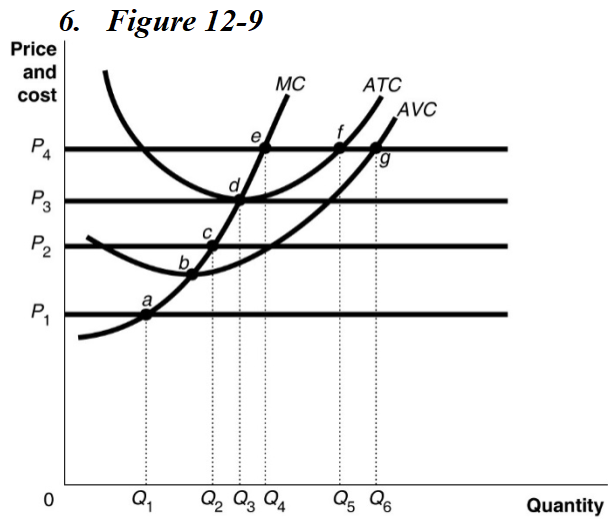
\includegraphics[scale=.6]{images/graph.png}
    \end{center}
    \newline
    Figure 12-9 shows cost and demand curves facing a profit-maximizing, perfectly competitive firm. At price $P1$, the firm would produce?
\end{frame}

\begin{frame}[t]{PC Firms}
    \begin{center}
        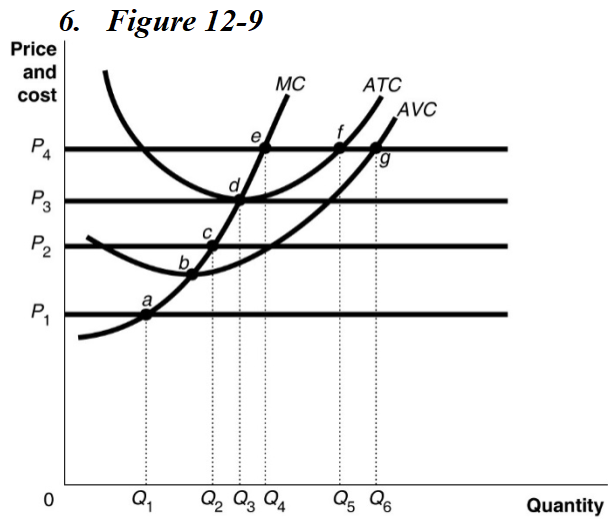
\includegraphics[scale=.6]{images/graph.png}
    \end{center}
    \newline
    Figure 12-9 shows cost and demand curves facing a profit-maximizing, perfectly competitive firm. At price $P1$, the firm would lose an amount (more than/less than/equal to) their fixed cost.
\end{frame}

\begin{frame}[t]{PC Firms}
    \begin{center}
        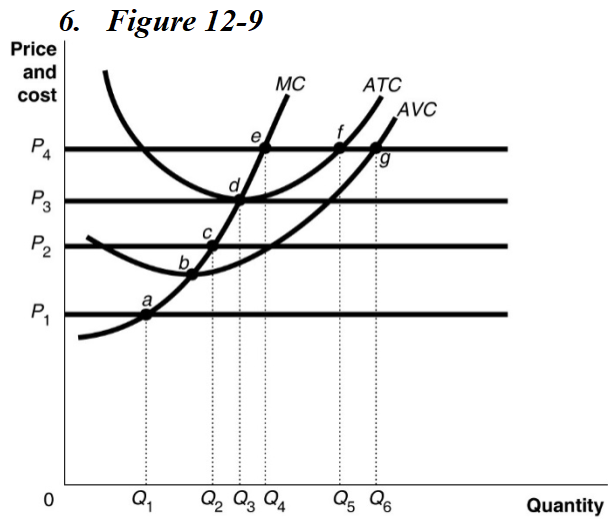
\includegraphics[scale=.6]{images/graph.png}
    \end{center}
    \newline
    Figure 12-9 shows cost and demand curves facing a profit-maximizing, perfectly competitive firm. At price $P2$, the firm would produce?
\end{frame}

\begin{frame}[t]{PC Firms}
    \begin{center}
        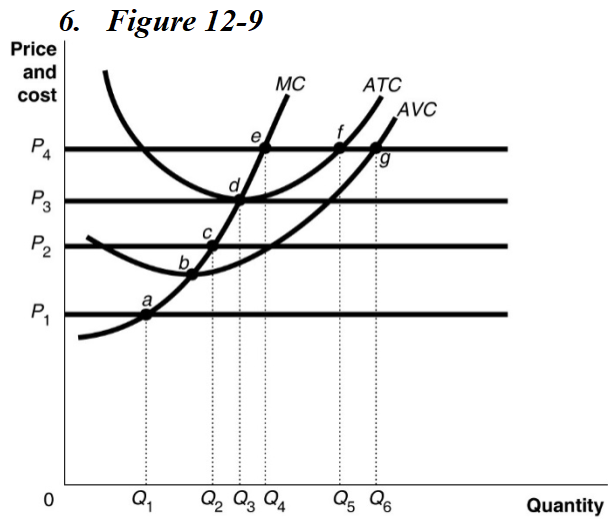
\includegraphics[scale=.6]{images/graph.png}
    \end{center}
    \newline
    Figure 12-9 shows cost and demand curves facing a profit-maximizing, perfectly competitive firm. At price $P2$, the firm would lose an amount (more than/less than/equal to) their fixed cost.
\end{frame}

\begin{frame}[t]{PC Firms}
    \begin{center}
        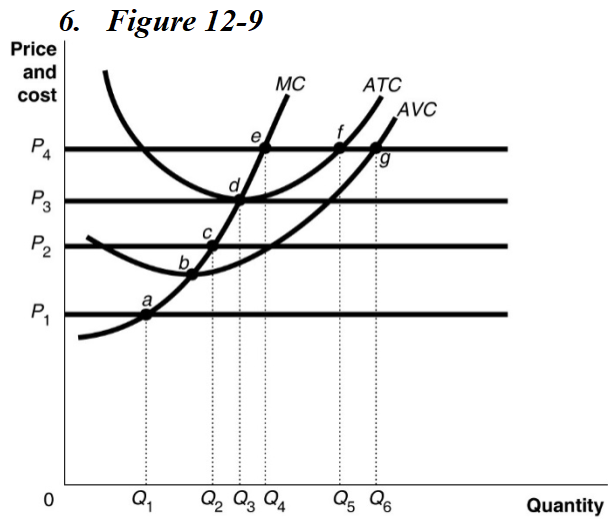
\includegraphics[scale=.6]{images/graph.png}
    \end{center}
    \newline
    Figure 12-9 shows cost and demand curves facing a profit-maximizing, perfectly competitive firm. At price $P3$, the firm would produce?
\end{frame}

\begin{frame}[t]{PC Firms}
    \begin{center}
        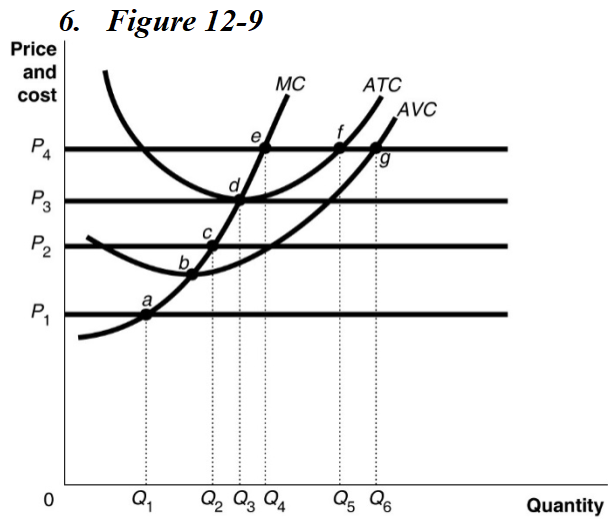
\includegraphics[scale=.6]{images/graph.png}
    \end{center}
    \newline
    Figure 12-9 shows cost and demand curves facing a profit-maximizing, perfectly competitive firm. At price $P3$, the firm profits would be?
\end{frame}

\begin{frame}[t]{PC Firms}
    \begin{center}
        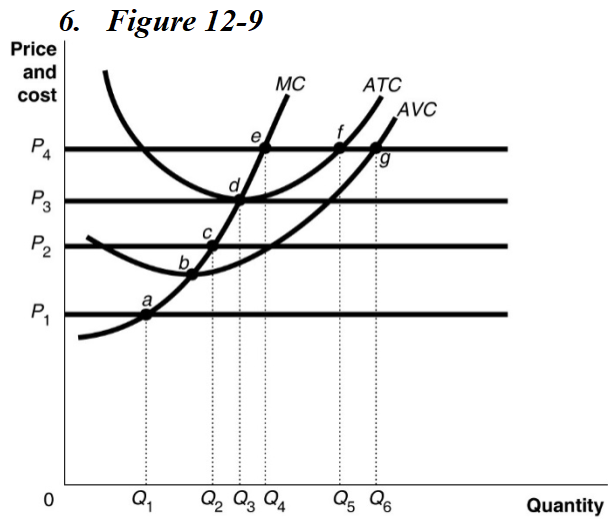
\includegraphics[scale=.6]{images/graph.png}
    \end{center}
    \newline
    Figure 12-9 shows cost and demand curves facing a profit-maximizing, perfectly competitive firm. At price $P4$, the firm would produce?
\end{frame}

\begin{frame}[t]{PC Firms}
    \begin{center}
        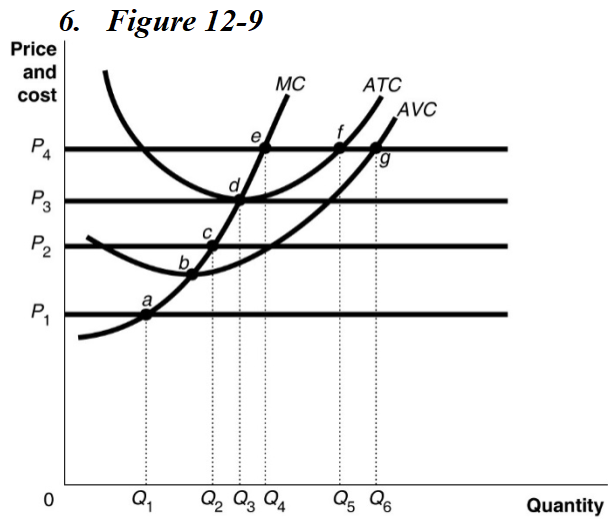
\includegraphics[scale=.6]{images/graph.png}
    \end{center}
    \newline
    Figure 12-9 shows cost and demand curves facing a profit-maximizing, perfectly competitive firm. At price $P4$, the firm’s profits would be (positive/negative).
\end{frame}

\begin{frame}[t]{PC Firms}
    \begin{center}
        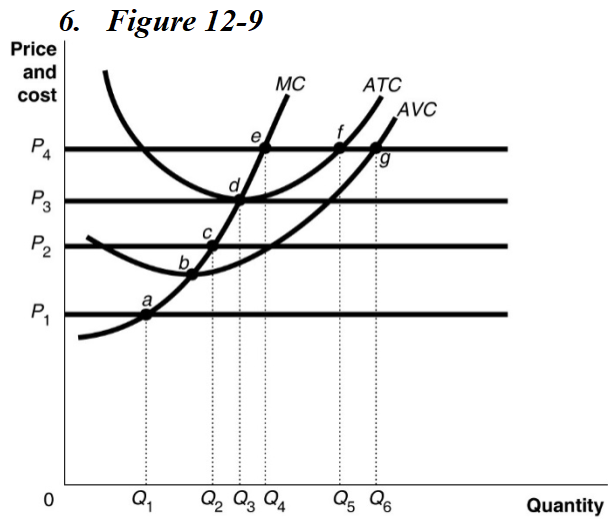
\includegraphics[scale=.6]{images/graph.png}
    \end{center}
    \newline
    Figure 12-9 shows cost and demand curves facing a profit-maximizing, perfectly competitive firm. Identify the short-run shut down point for the firm.
\end{frame}

\begin{frame}[t]{PC Firms}
    \begin{center}
        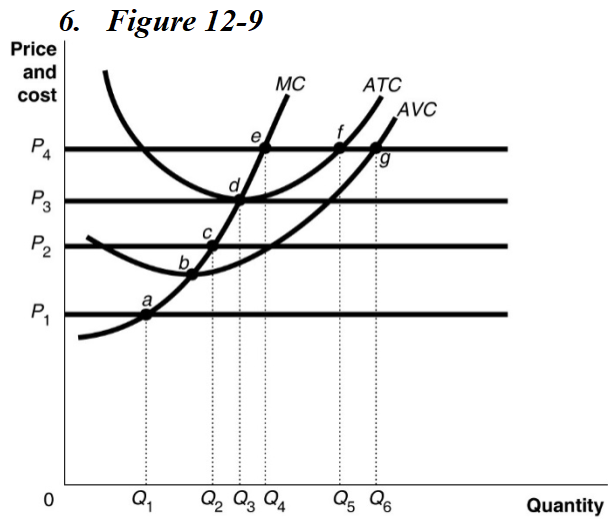
\includegraphics[scale=.6]{images/graph.png}
    \end{center}
    \newline
    Which of the following identifies the firm's short-run supply curve?
    \begin{itemize}
        \item the MC curve
        \item the MC curve from $a$ and above
        \item the MC curve from $b$ and above
        \item the MC curve from $d$ and above
    \end{itemize}
\end{frame}

\begin{frame}{LR vs SR}
    A perfectly competitive market see an increase in demand from $D_1$ to $D_2$
    \begin{center}
    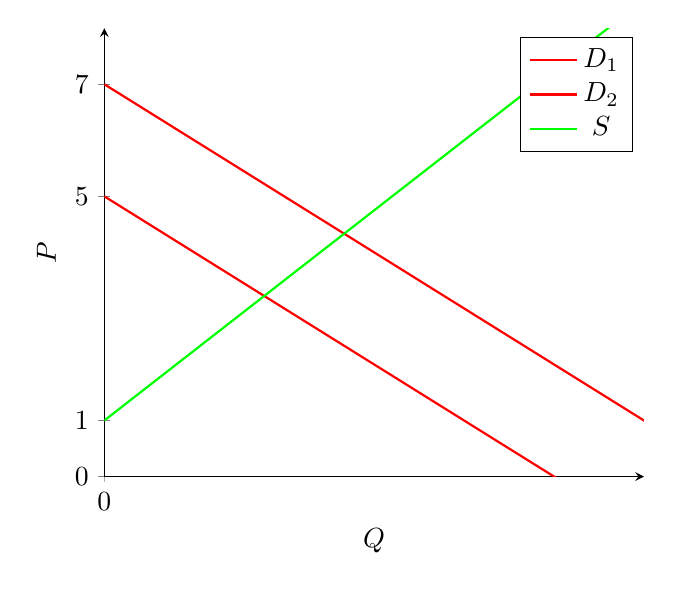
\begin{tikzpicture}
    \begin{axis}[
        axis lines = left,
        xlabel = $Q$,
        ylabel = $P$,
        ymax = 8,
        ymin = 0,
        xmax = 30,
        xmin = 0,
        scaled x ticks = false,
        ytick = {0,1,5,7},
        xtick = {0}
    ]
    \addplot[
    color=red,thick,
    domain=0:50,
    range = 0:50]{-x/5 + 5};
    \addlegendentry{{$D_1$}}
    \addplot[
    color=red,thick,
    domain=0:50,
    range = 0:50]{-x/5 + 7};
    \addlegendentry{{$D_2$}}
    \addplot[
    color=green,thick,
    domain=0:50,
    range = 0:50]{x/4 + 1};
    \addlegendentry{$S$}
    % \addplot[
    % color=blue,thick,dashed,
    % domain=0:50,
    % range = 0:50]{1.5};
    % \addlegendentry{{World Price ($P_W$)}}
    % \addplot[
    % color=blue,thick,dotted,
    % domain=0:50,
    % range = 0:50]{2};
    % \addlegendentry{{$P_W$ + Tariff}}
    \end{axis}
    \end{tikzpicture}
\end{center}
\end{frame}

\begin{frame}{LR vs SR}
    \begin{center}
    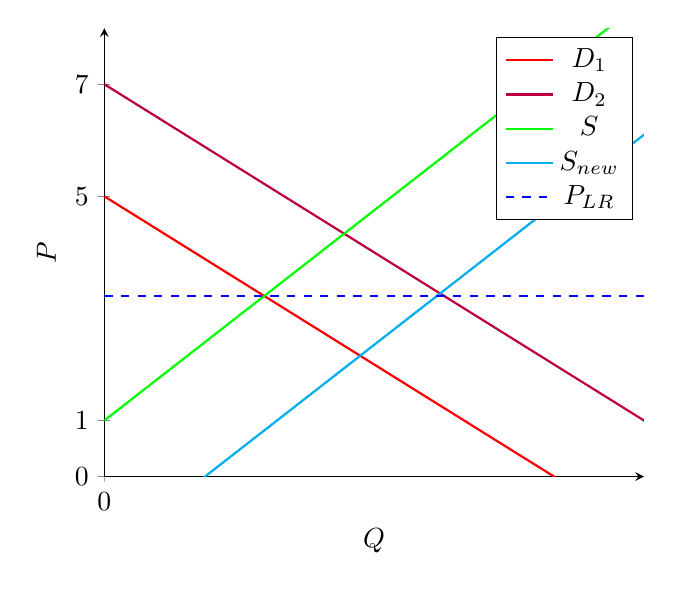
\begin{tikzpicture}
    \begin{axis}[
        axis lines = left,
        xlabel = $Q$,
        ylabel = $P$,
        ymax = 8,
        ymin = 0,
        xmax = 30,
        xmin = 0,
        scaled x ticks = false,
        ytick = {0,1,5,7},
        xtick = {0}
    ]
    \addplot[
    color=red,thick,
    domain=0:50,
    range = 0:50]{-x/5 + 5};
    \addlegendentry{{$D_1$}}
    \addplot[
    color=purple,thick,
    domain=0:50,
    range = 0:50]{-x/5 + 7};
    \addlegendentry{{$D_2$}}
    \addplot[
    color=green,thick,
    domain=0:50,
    range = 0:50]{x/4 + 1};
    \addlegendentry{$S$}
    \addplot[
    color=cyan,thick,
    domain=0:50,
    range = 0:50]{x/4 -1.4};
    \addlegendentry{$S_{new}$}
    \addplot[
    color=blue,thick,dashed,
    domain=0:50,
    range = 0:50]{29/9};
    \addlegendentry{{$P_{LR}$}}
    % \addplot[
    % color=blue,thick,dotted,
    % domain=0:50,
    % range = 0:50]{2};
    % \addlegendentry{{$P_W$ + Tariff}}
    \end{axis}
    \end{tikzpicture}
\end{center}
\end{frame}

\begin{frame}{Firm Decisions}
    \begin{center}
        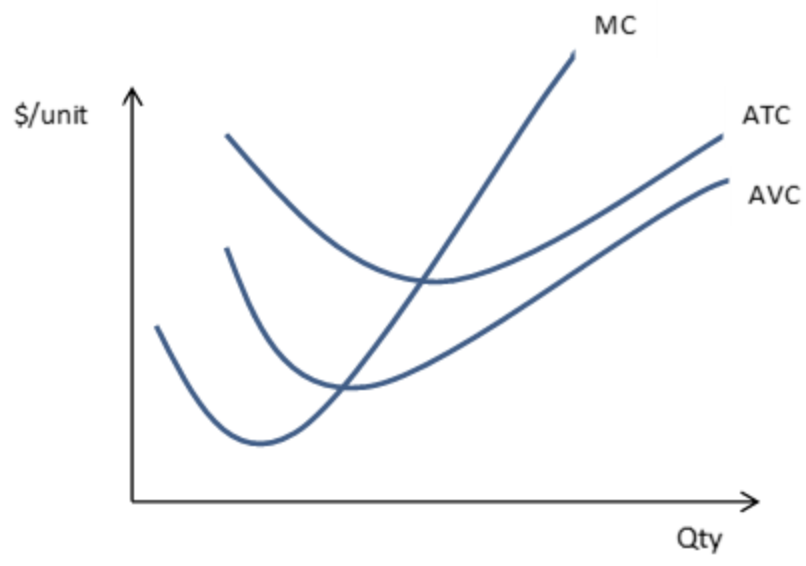
\includegraphics[scale = .6]{images/less_nice_graph.png}
    \end{center}
\end{frame}

\begin{frame}{Practice Final 2019 Q1}
    \begin{table}[]
    \begin{tabular}{ccccccc}
    L & Q   & MPL & TC & MC & ATC & AVC \\ \hline
    1 & 50  &     &    &    &     &     \\ \hline
    2 & 100 &     &    &    &     &     \\ \hline
    3 & 140 &     &    &    &     &     \\ \hline
    4 & 160 &     &    &    &     &     \\ \hline
    5 & 175 &     &    &    &     &     \\ \hline
    6 & 185 &     &    &    &     &    
    \end{tabular}
    \end{table}
    Sherry’s is a profit maximizing firm in a perfectly competitive market, and a worker earns \$100 per day.  Fixed costs come from a 1-year contract for rents paid on the farmer’s market stall, and are \$200 per day. In the table above, find the MPL, TC, MC, ATC and AVC.  No need to show your work. 
\end{frame}

\begin{frame}{Practice Final 2019 Q1}
    \begin{table}[]
    \begin{tabular}{ccccccc}
    L & Q   & MPL & TC & MC & ATC & AVC \\ \hline
    1 & 50  &     &    &    &     &     \\ \hline
    2 & 100 &     &    &    &     &     \\ \hline
    3 & 140 &     &    &    &     &     \\ \hline
    4 & 160 &     &    &    &     &     \\ \hline
    5 & 175 &     &    &    &     &     \\ \hline
    6 & 185 &     &    &    &     &    
    \end{tabular}
    \end{table}
    If the market price of cherries is \$5/pound this summer, how much output would Sherry’s produce per day?  Calculate the daily profits at this level of output. Show your work. 
\end{frame}

\begin{frame}{Practice Final 2019 Q1}
    \begin{table}[]
    \begin{tabular}{ccccccc}
    L & Q   & MPL & TC & MC & ATC & AVC \\ \hline
    1 & 50  &     &    &    &     &     \\ \hline
    2 & 100 &     &    &    &     &     \\ \hline
    3 & 140 &     &    &    &     &     \\ \hline
    4 & 160 &     &    &    &     &     \\ \hline
    5 & 175 &     &    &    &     &     \\ \hline
    6 & 185 &     &    &    &     &    
    \end{tabular}
    \end{table}
    What output would be produced if prices fell to \$1.75/ pound the following year? What would her profits be in the short run?
\end{frame}

\begin{frame}{Practice Final 2019 Q1}
    On the graph below, draw the marginal revenue for if the firm is in a perfectly competitive market and making positive profits. Indicate the firm’s output.
    \begin{center}
        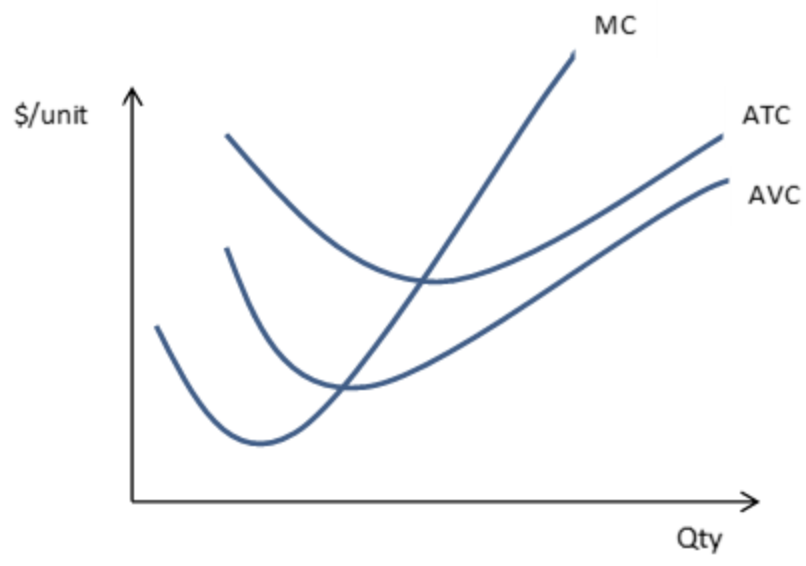
\includegraphics[scale = .6]{images/less_nice_graph.png}
    \end{center}
\end{frame}

\end{document}
